\documentclass{article}
% 2D and 3D plots: pgfplots (surface, mesh, quiver, polar, fill between,
% group plots, data from a table), tikz-3dplot, and a 3D-ish TikZ drawing.
\usepackage{pgfplots}
\pgfplotsset{compat=1.18}
\usepgfplotslibrary{fillbetween,polar,groupplots,colormaps}
\usepackage{pgfplotstable}
\usepackage{tikz-3dplot}
\usetikzlibrary{3d,calc,arrows.meta,perspective}
\usepackage{filecontents}
\usepackage[margin=2cm]{geometry}

\begin{filecontents*}{data.csv}
x,y,err
0,1.0,0.1
1,2.1,0.2
2,3.9,0.15
3,9.2,0.3
4,15.8,0.4
\end{filecontents*}

\begin{document}
\section{2D}
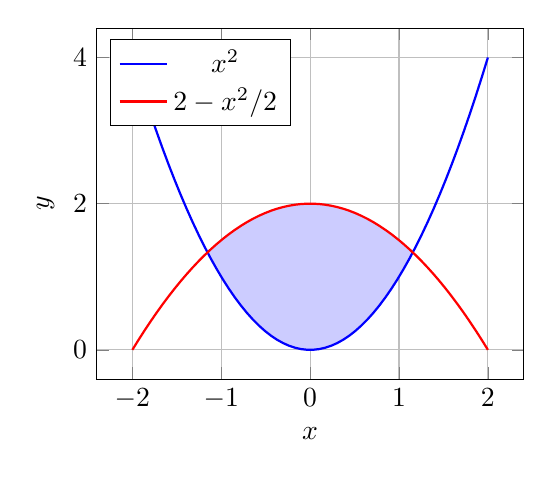
\begin{tikzpicture}
  \begin{axis}[width=7cm, xlabel=$x$, ylabel=$y$, legend pos=north west, grid=major]
    \addplot[name path=f, blue, thick, domain=-2:2, samples=60] {x^2};
    \addplot[name path=g, red, thick, domain=-2:2, samples=60] {2-x^2/2};
    \addplot[blue!20] fill between[of=f and g, soft clip={domain=-1.15:1.15}];
    \addlegendentry{$x^2$}
    \addlegendentry{$2-x^2/2$}
  \end{axis}
\end{tikzpicture}
\begin{tikzpicture}
  \begin{axis}[width=7cm, ymode=log, xlabel=$t$, ylabel=value]
    \addplot+[error bars/.cd, y dir=both, y explicit] table[x=x, y=y, y error=err, col sep=comma] {data.csv};
  \end{axis}
\end{tikzpicture}

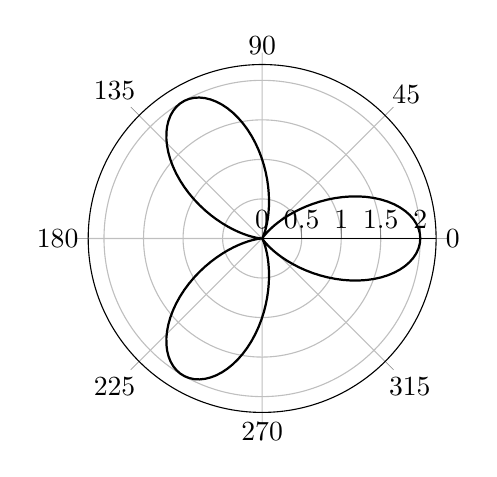
\begin{tikzpicture}
  \begin{polaraxis}[width=6cm]
    \addplot[domain=0:360, samples=200, thick] {1+cos(3*x)};
  \end{polaraxis}
\end{tikzpicture}
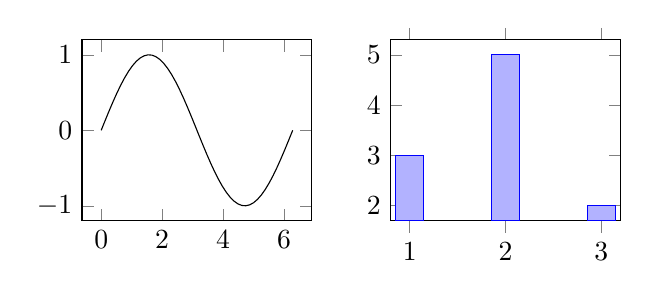
\begin{tikzpicture}
  \begin{groupplot}[group style={group size=2 by 1}, width=4.5cm]
    \nextgroupplot \addplot[domain=0:2*pi, samples=50] {sin(deg(x))};
    \nextgroupplot[ybar] \addplot coordinates {(1,3) (2,5) (3,2)};
  \end{groupplot}
\end{tikzpicture}

\pgfplotstabletypeset[col sep=comma, columns/err/.style={fixed, precision=2}]{data.csv}

\section{3D}
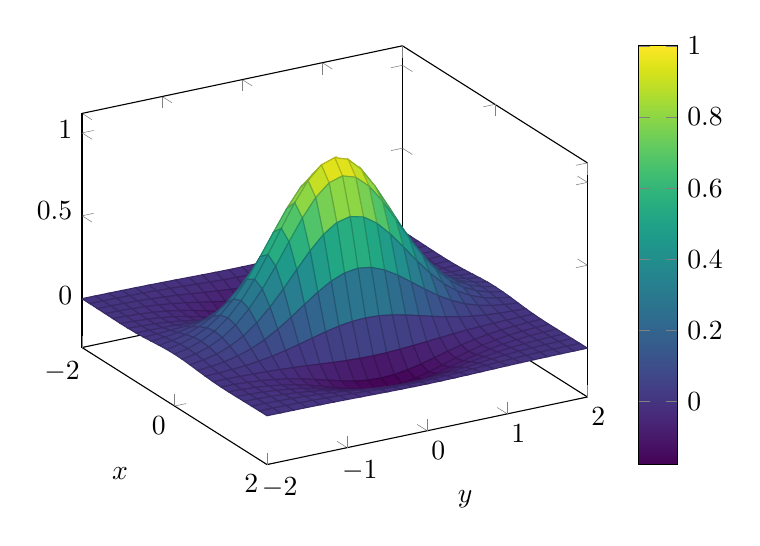
\begin{tikzpicture}
  \begin{axis}[width=8cm, view={60}{30}, colormap/viridis, colorbar, xlabel=$x$, ylabel=$y$]
    \addplot3[surf, domain=-2:2, samples=25] {exp(-x^2-y^2)*cos(deg(2*x))};
  \end{axis}
\end{tikzpicture}
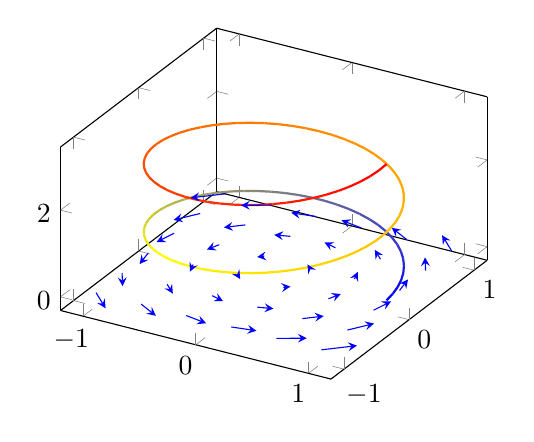
\begin{tikzpicture}
  \begin{axis}[width=7cm, view={30}{40}]
    \addplot3[mesh, domain=0:4*pi, samples y=0, samples=120, thick] ({cos(deg(x))}, {sin(deg(x))}, {x/4});
    \addplot3[quiver={u=-y, v=x, w=0, scale arrows=0.2}, -stealth, samples=6, domain=-1:1, blue] {0};
  \end{axis}
\end{tikzpicture}

\tdplotsetmaincoords{70}{110}
\begin{tikzpicture}[tdplot_main_coords, scale=2]
  \draw[thick,->] (0,0,0) -- (1.2,0,0) node[anchor=north east]{$x$};
  \draw[thick,->] (0,0,0) -- (0,1.2,0) node[anchor=north west]{$y$};
  \draw[thick,->] (0,0,0) -- (0,0,1.2) node[anchor=south]{$z$};
  \tdplotsetcoord{P}{1}{50}{60}
  \draw[-stealth, red, thick] (0,0,0) -- (P) node[above right]{$P$};
  \draw[dashed] (0,0,0) -- (Pxy) -- (P);
  \tdplotdrawarc{(0,0,0)}{0.3}{0}{60}{anchor=north}{$\phi$}
\end{tikzpicture}
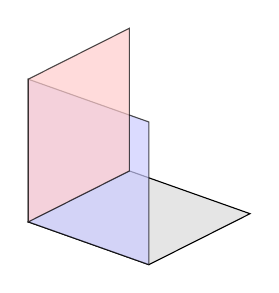
\begin{tikzpicture}[3d view={40}{25}]
  \draw[canvas is xy plane at z=0, fill=gray!20] (0,0) rectangle (2,2);
  \draw[canvas is xz plane at y=0, fill=blue!20, opacity=0.7] (0,0) rectangle (2,2);
  \draw[canvas is yz plane at x=0, fill=red!20, opacity=0.7] (0,0) rectangle (2,2);
\end{tikzpicture}
\end{document}
